\chapter{Lo que se lee de las simulaciones}
\label{cap:lectura}

Las 20.000 temporadas simuladas son una muestra de la distribución conjunta de todos los resultados pendientes y de la tabla final. La matriz de posiciones es solo su marginal más visible. Este capítulo describe cuatro cantidades más que salen de la misma muestra, y una técnica para estimar probabilidades demasiado chicas para verlas en ella.

\section{La importancia de un partido como información mutua}
\label{sec:mi}

Sea $O_k\in\{L,E,V\}$ el resultado de un partido pendiente y $F$ una variable de la tabla final: el campeón $C$ o el indicador de descenso $R_i$ de cada equipo. Se define la importancia del partido como
\[
\mathcal I_k^{\text{título}}=I(O_k;C),\qquad \mathcal I_k^{\text{descenso}}=\sum_i I(O_k;R_i),
\]
en bits. Es cuánta incertidumbre sobre el desenlace resuelve, en promedio, saber el resultado de ese partido.

\begin{proposicion}[Propiedades] \dem
$0\le I(O_k;C)\le\min\{H(O_k),H(C)\}\le\log_23$. Vale cero si y solo si el resultado es independiente del campeón, y es invariante a reetiquetar resultados.
\end{proposicion}

\begin{proof}
Son propiedades generales de la información mutua: $I(X;Y)=H(X)-H(X\mid Y)\le H(X)$ y es simétrica, $H(O_k)\le\log_2 3$ porque $O_k$ toma tres valores, y $I(X;Y)=0$ si y solo si la distribución conjunta es el producto de las marginales.
\end{proof}

Se estima con las mismas simulaciones: cada una trae el resultado de cada partido pendiente y la tabla final. El estimador por frecuencias tiene un sesgo positivo, que se corrige con Miller–Madow~\cite{miller1955}: $\hat I-(|O|-1)(|F|-1)/(2S\ln2)$. A diferencia de las medidas clásicas de importancia, que fijan un umbral o un evento (``el partido es importante si puede cambiar al campeón''), no hay nada que elegir. El sitio lista los seis partidos más importantes de cada liga, separando título y descenso.

\section{¿Qué necesita mi equipo?}
\label{sec:necesita}

La ficha de cada equipo muestra la curva $p(g)=P(\text{objetivo}\mid\text{suma }g\text{ puntos desde hoy})$ y los $g$ con $p\ge0{,}5$ y $p\ge0{,}9$, para el título, la clasificación a copas, el ascenso o salvarse. Contar éxitos entre las temporadas simuladas en que el equipo sumó exactamente $g$ es exacto, pero solo donde hay simulaciones. Un equipo muy superior casi nunca suma pocos puntos y uno modesto casi nunca gana todo: con la regla ``mínimo $g$ con 30 simulaciones'', el Real Madrid ``necesitaba'' 41 puntos para salvarse y el Betis ``no salía campeón ni ganando todo''. Donde hay pocas simulaciones, además, la curva sale con saltos que son ruido de Monte Carlo.

\begin{proposicion}[Remuestreo condicional] \dem
Sean $r=(r_1,\dots,r_K)$ los resultados de los $K$ partidos que le quedan al equipo y $x$ las fuerzas de una temporada simulada. Para la familia inclinada
\[
q_\vartheta(r\mid x)\propto p(r\mid x)\,e^{\vartheta\,g(r)},\qquad g(r)=\text{puntos del equipo},
\]
se cumple $q_\vartheta(r\mid g(r)=g,\,x)=p(r\mid g(r)=g,\,x)$ para todo $\vartheta$.
\end{proposicion}

\begin{proof}
Para $r$ con $g(r)=g$, $q_\vartheta(r\mid x)=p(r\mid x)e^{\vartheta g}/Z_\vartheta(x)$. Al condicionar en $g(r)=g$ el factor $e^{\vartheta g}/Z_\vartheta(x)$ es constante y se cancela en la normalización.
\end{proof}

La inclinación depende solo del total $g$, así que, condicionada a un total, deja intacta la distribución de \emph{qué} partidos gana. En cada temporada simulada se vuelven a sortear solo esos $K$ resultados, para una grilla de $\vartheta$ que lleva el total desde casi cero hasta casi todos los puntos. Dado el estado, los partidos son independientes, así que el resto de la temporada sigue siendo una muestra válida. Los rivales ganan o pierden esos mismos partidos y la tabla se reordena (desempate: el orden original de esa simulación). Dentro de cada $g$ todas las muestras valen lo mismo y se juntan entre valores de $\vartheta$: hay miles en cada punto de la curva. Lo único que no se ajusta es la fuerza del propio equipo dado $g$, que solo pesa por su correlación posterior con la de los demás. Finalmente se impone que la curva no baje con $g$ con una regresión isotónica~\cite{barlow1972}.

\begin{figure}[h]
\centering
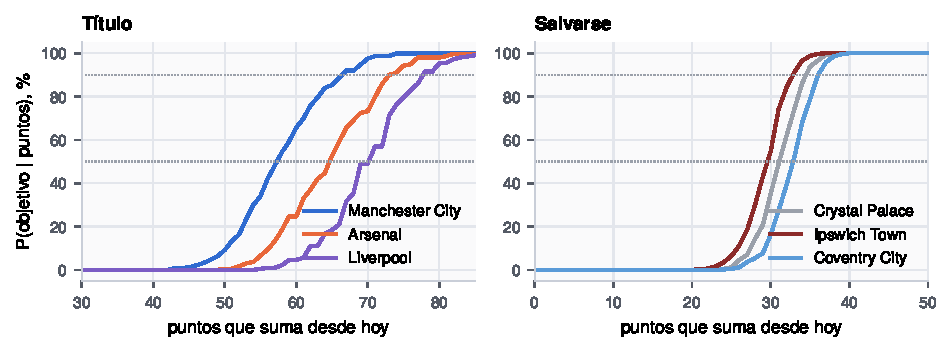
\includegraphics[width=\textwidth]{necesita}
\caption{Curvas de ``qué necesita'' en la Premier 2026-27 tras 65 partidos: probabilidad de salir campeón (izquierda) y de salvarse (derecha) según los puntos que el equipo sume desde hoy. Las líneas punteadas marcan 50\,\% y 90\,\%.}
\label{fig:necesita}
\end{figure}

Con esto, los puntos finales que dan 50\,\% de salvarse coinciden entre los equipos de cada liga: Premier 38-39, LaLiga 36-38, Serie A 35-36, Bundesliga 30-32, Ligue 1 30-31, Championship 46-48. Los del título difieren con razón, porque dependen de a quién hay que superar: al Bayern le bastan 70 y a los demás 82-83. Los escalones que quedan en la curva del título son reales, porque los rivales suman de a 3 y de a 1.

Cuando el objetivo se define en una llave (ganar el torneo argentino o una copa), la fase regular solo decide si se entra al cuadro, el cruce y la localía: ni ganando todo se llega al 50\,\%, y la lectura ``con $g$ puntos lo logra en la mitad de las simulaciones'' no tiene sentido. Para esos objetivos la ficha muestra la curva con su propia escala, el máximo $p(g_{\max})$ frente a la probabilidad de hoy, y el primer $g$ con $p(g)\ge p(g_{\max})/2$.

\section{Cotas matemáticas}

Que un equipo ``ya no pueda'' salir campeón no es una afirmación probabilística. Con puntuación 3-1-0, decidir si un equipo todavía puede terminar primero es NP-completo~\cite{kern2001}, así que la mejor y la peor posición posibles se calculan como programas enteros (HiGHS):
\[
\text{mejor}(i)=1+\min_{x}\#\{j:P_j(x)>P_i(x)\},\qquad \text{peor}(i)=1+\max_x\#\{j:P_j(x)\ge P_i(x)\},
\]
con $x$ las variables binarias de resultado de cada partido pendiente y los indicadores linealizados con big-M. Los empates en puntos se tratan a favor (para la mejor) y en contra (para la peor), porque la diferencia de gol no está acotada por los puntos: las cotas son conservadoras. Con ellas el sitio marca ``campeón'', ``eliminado del título'', ``descendido'' y ``salvado'' solo cuando es matemáticamente cierto.

\section{Suspenso}

Con la secuencia de creencias $\mu_t$ sobre el campeón a lo largo de la temporada se miden dos cosas. La entropía $H(\mu_t)$ es la incertidumbre que queda; la \emph{sorpresa} de Ely, Frankel y Kamenica~\cite{ely2015}, $\sum_t\|\mu_t-\mu_{t-1}\|_2^2$, cuánto se movieron las creencias. Se reportan junto a medidas estáticas de equilibrio competitivo: HHI normalizado, Gini y Noll–Scully con empates, que es la desviación de puntos por partido dividida por la de una liga de equipos iguales con la misma tasa de empates. Los resultados están en la sección~\ref{sec:r11}.

\section{Eventos casi imposibles}
\label{sec:raros}

¿Qué probabilidad tiene el Manchester City de descender? Con $n$ temporadas simuladas el error relativo de Monte Carlo es $\sqrt{(1-p)/(np)}$: para $p=10^{-6}$ y un 10\,\% de error harían falta $10^8$ temporadas. Un evento extremo de un equipo ocurre combinando dos caminos: que el equipo \emph{sea} peor de lo que se cree y que le vaya mal. La propuesta de muestreo por importancia inclina ambos:
\begin{itemize}
\item \textbf{la fuerza}: el bloque $w=(a_t,b_t)$ del equipo se sortea de $\N(\mu_w-c\,u,\,P_{ww})$, con $u$ la dirección que baja su fuerza neta en una desviación a priori, y el resto del estado de su condicional exacta dado $w$;
\item \textbf{los resultados}: en cada partido del equipo su tasa de goles se multiplica por $e^{-\vartheta}$ y la del rival por $e^{\vartheta}$.
\end{itemize}

\begin{proposicion}[Razón de verosimilitudes] \dem
Con $A$ el evento de interés,
\[
W=\frac{\N(w;\mu_w,P_{ww})}{\N(w;\mu_w-cu,P_{ww})}\prod_{m\ni t}\frac{p(x_m,y_m;\lambda_m,\nu_m)}{p(x_m,y_m;\lambda_me^{-\vartheta},\nu_me^{\vartheta})},
\]
el estimador $\hat p=\tfrac1n\sum_kW_k\,\ind\{A_k\}$ es insesgado: $\E_q[\hat p]=p$.
\end{proposicion}

\begin{proof}
La ley propuesta y la original difieren solo en la densidad de $w$ (el resto del estado se sortea de la misma condicional dado $w$) y en la de los partidos del equipo $t$. Todo lo demás (el paseo aleatorio, los otros partidos, los desempates) es idéntico bajo ambas. La derivada de Radon–Nikodym es entonces el producto de esos cocientes, y $\E_q[W\ind_A]=\E_p[\ind_A]$.
\end{proof}

Los parámetros $(c,\vartheta)$ se eligen en corridas piloto minimizando la varianza relativa estimada, $\E_q[W^2\ind_A]/\E_q[W\ind_A]^2-1$.

\begin{nota}{Lo que no funcionó}
Inclinar solo el estado, con el método de entropía cruzada~\cite{rubinstein2004} y también con mezclas y covarianza adaptada, da estimadores de cola pesada para $p\sim10^{-7}$: tamaños efectivos de 1 a 7 y semillas que discrepan en órdenes de magnitud. La mala suerte sin inclinar casi nunca se muestrea, y es parte del camino dominante hacia el evento.
\end{nota}
